
\subsection{What's グラフ?}
\frame{
  \frametitle{グラフ}
  \begin{block}{graph}
    \alert{グラフ}は有限集合$V,E$と関数$\Psi$の3つ組で定義され,\\ \\
    無向グラフの場合,
    \[ \Psi: E \rightarrow \{ X \subset V : |X| = 2 \} \]
    有向グラフの場合,
    \[ \Psi: E \rightarrow V \times V\]
     
  \end{block}
}

\frame{
  \begin{exampleblock}{グラフの例}
    左が有向グラフ,右が無向グラフ
    \center{
      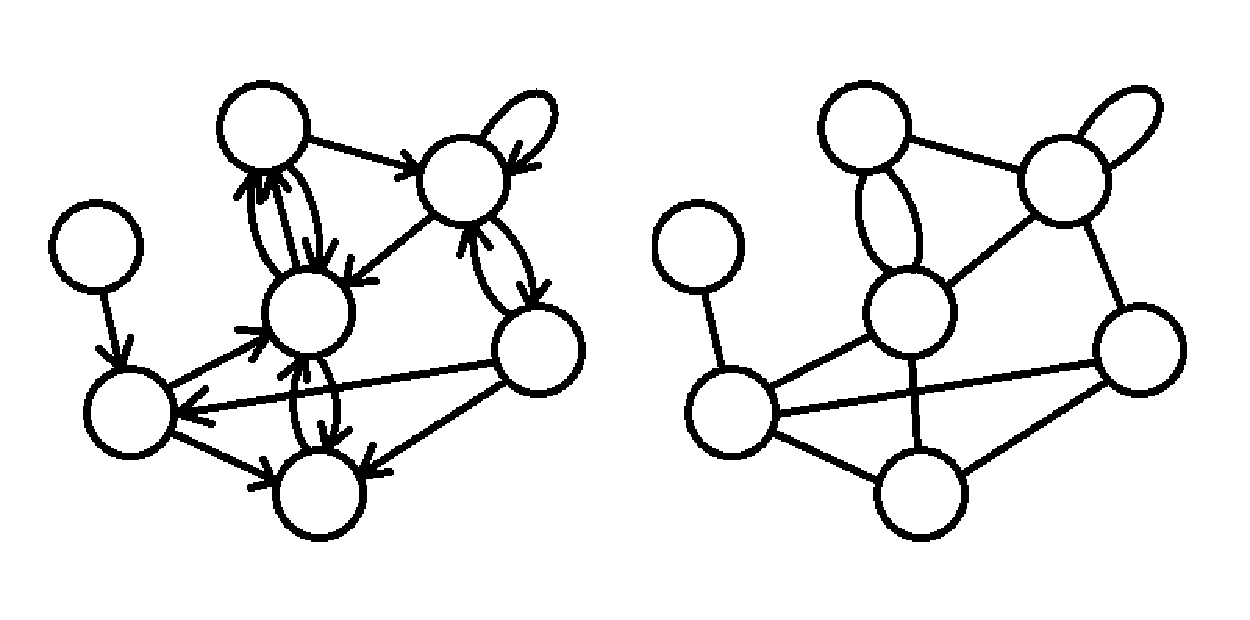
\includegraphics[width=8cm]{image/graph01.pdf}
    }
  \end{exampleblock}
}
    
\subsection{単純グラフ}
\frame{
  \frametitle{単純グラフ}
  \begin{block}{simple graph}
    自己ループと多重辺を持たないグラフを\alert{単純グラフ}という.\\
    通常,$e$と$\Psi(e)$を同一視して,\\ \\
    無向グラフの場合,
    \[ E(G) \subset \{ X \subset V(G) : |X| = 2 \} \]
    有向グラフの場合,
    \[ E(G) \subset \{(v,w) \in V(G) \times V(G) : v \neq w \} \]
    を用いて,$G=(V(G),E(G))$と書く.
  \end{block}
}

\frame{
  \begin{exampleblock}{単純グラフの例}
    左が有向グラフ,右が無向グラフ
    \center{
      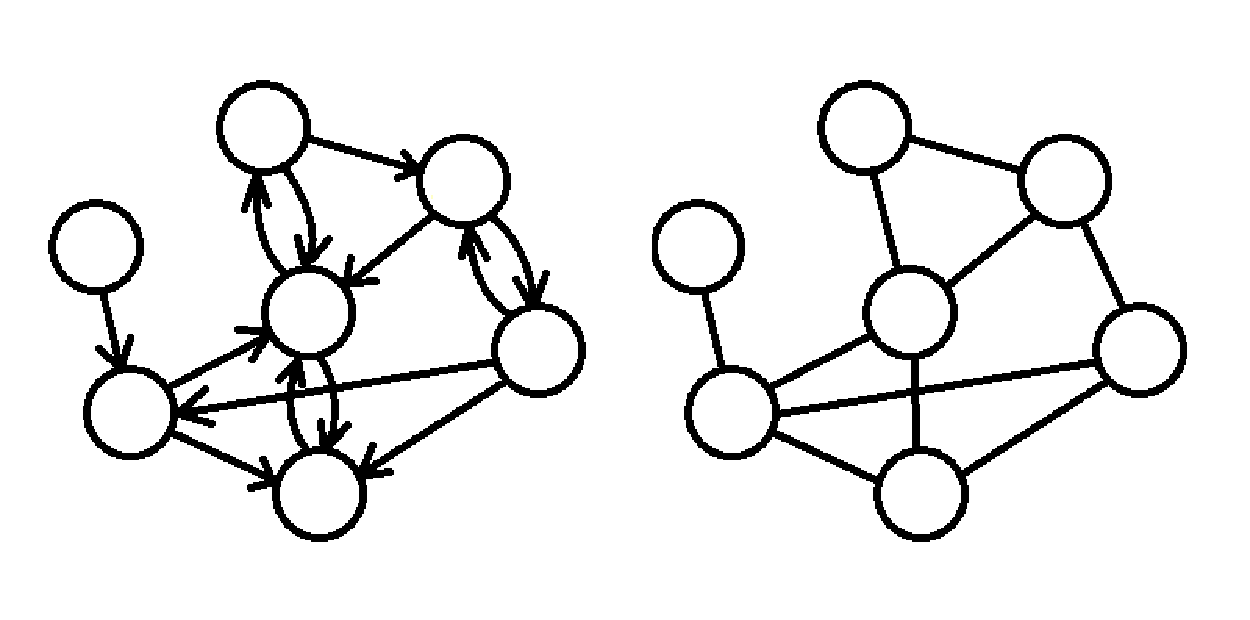
\includegraphics[width=8cm]{image/graph02.pdf}
    }
  \end{exampleblock}
}
    
\subsection{部分グラフ}
\frame{
  \frametitle{部分グラフ}
  \begin{block}{subgraph}
    グラフ$G=(V(G),E(G))$に対して,
    \[ V(H) \subset V(G) ~~ and ~~ E(H) \subset E(G) \]
    となる$H=(V(H),E(H))$をGの\alert{部分グラフ}という.\\
    このとき$G$は$H$を含むともいう.
  \end{block}
}

\frame{
  \begin{exampleblock}{部分グラフの例}
    左が有向グラフ,右が無向グラフ
    \center{
      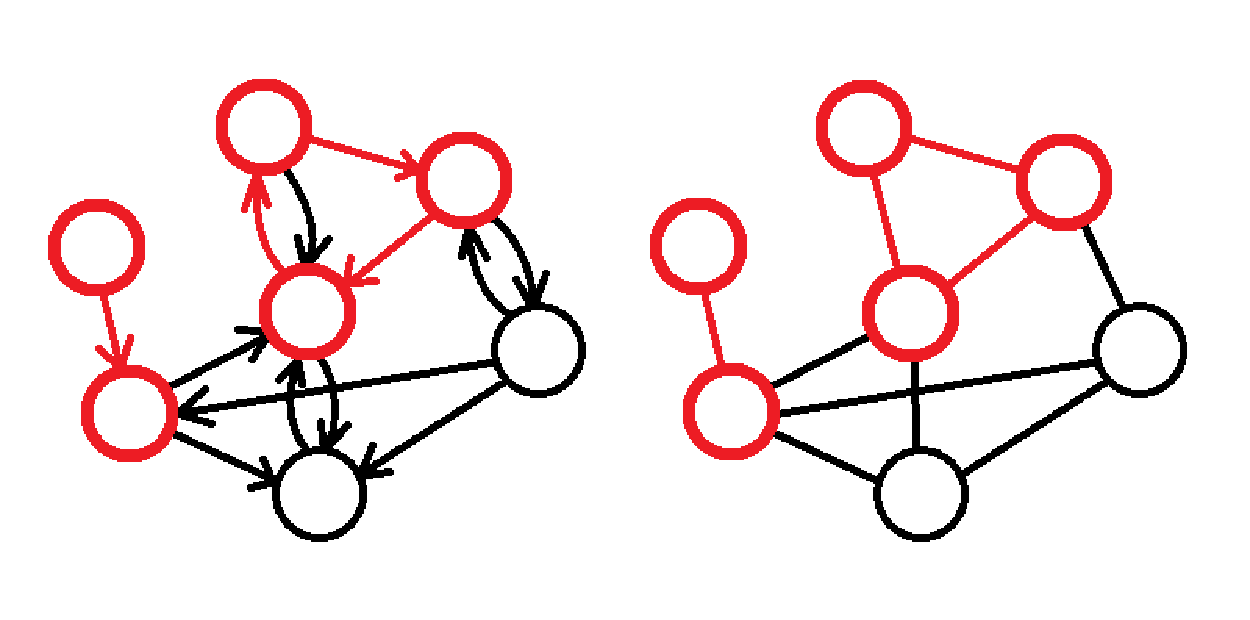
\includegraphics[width=8cm]{image/graph03.pdf}
    }
  \end{exampleblock}
}

\subsection{全点}
\frame{
  \frametitle{全点}
  \begin{block}{spanning}
    グラフ$G$の部分グラフ$H$が,
    \[ V(G) = V(H) \]
    を満たすとき,$H$を$G$の\alert{全点}という.
  \end{block}
}

\frame{
  \begin{exampleblock}{全点の例}
    左が有向グラフ,右が無向グラフ
    \center{
      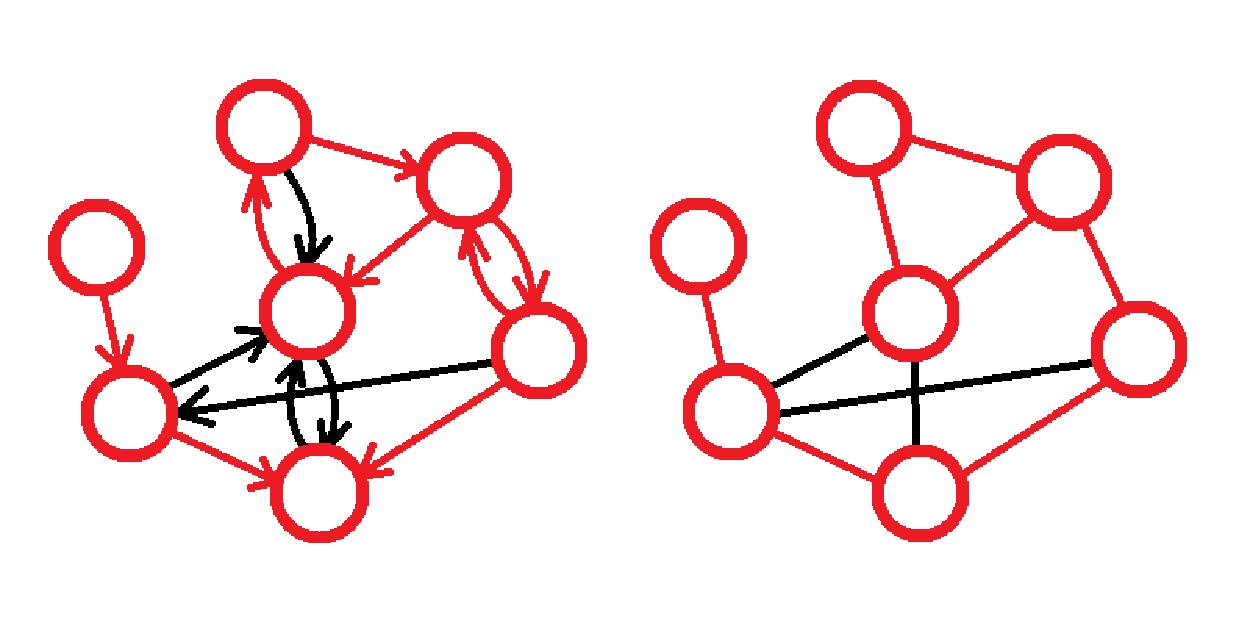
\includegraphics[width=8cm]{image/graph04.pdf}
    }
  \end{exampleblock}
}
    
\subsection{頂点の次数}
\frame{
  \frametitle{頂点の次数}
  \begin{block}{degree}
    無向グラフ$G$と$X,Y \subset V(G), ~ v \in V(G)$に対して,
    \[ E(X,Y) := \{ \{x,y\} \in E(G) : x \in X \backslash Y, y \in Y \backslash X \} \]
    \[ \delta(X) := E(X,V(G) \backslash X) \]
    \[ \delta(v) = \delta(\{v\}) \]
    と定義し,$|\delta(v)|$の値を点$v$の\alert{次数}という.
  \end{block}
}

\frame{
  \begin{block}{degree}
    有向グラフ$G$と$X,Y \subset V(G), ~ v \in V(G)$に対して,
    \[ E^+(X,Y) := \{ \{x,y\} \in E(G) : x \in X \backslash Y, y \in Y \backslash X \} \]
    \[ \delta^+(X) := E^+(X,V(G) \backslash X) \]
    \[ \delta^-(X) = \delta^+(V(G) \backslash X) \]
    \[ \delta(X) = \delta^+(X) \cup \delta^-(X) \]
    と定義し,$|\delta(v)|$の値を点$v$の\alert{次数}という.
  \end{block}
}

\frame{
  \begin{exampleblock}{例のグラフの次数}
    左が有向グラフ,右が無向グラフ
    \center{
      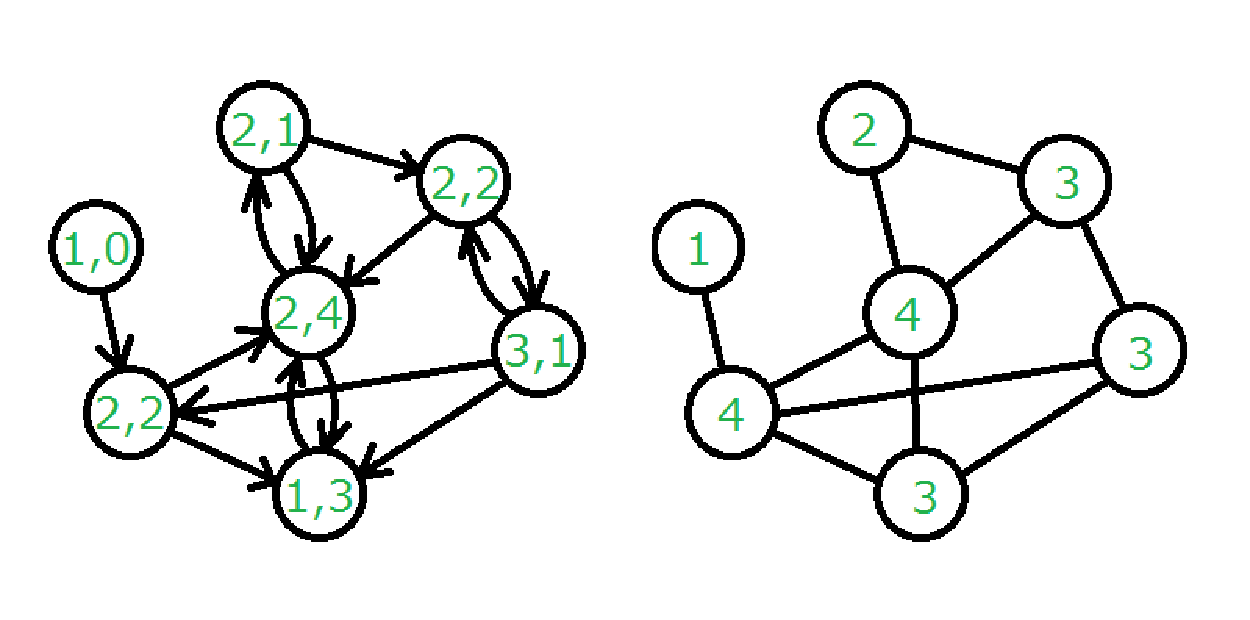
\includegraphics[width=8cm]{image/graph05.pdf}
    }
  \end{exampleblock}
}

\subsection{歩道と道}
\frame{
  \frametitle{歩道と道}
  \begin{block}{walk}
    グラフ$G$に対して,$G$の頂点と辺の有限個の交差系列
    \[ W = v_1, e_1, v_2, \cdots, v_k, e_k, v_{k+1} ~ (k \geq 0) \]
    が全ての$i=1,\cdots k$で$e_i=(v_i,v_{i+1})\in E(G)$\\
    (無向グラフの場合は$e_i=\{v_i,v_{i+1}\}\in E(G)$)を満たすとき,\\
    $W$をGの\alert{歩道}という.
  \end{block}
  \begin{block}{path}
    グラフ$G$に対して,$G$の歩道$W$の頂点がすべて異なるとき,\\
    $W$を$G$の\alert{道}という.
  \end{block}
}

\frame{
  \begin{exampleblock}{道の例}
    左が有向グラフ,右が無向グラフ
    \center{
      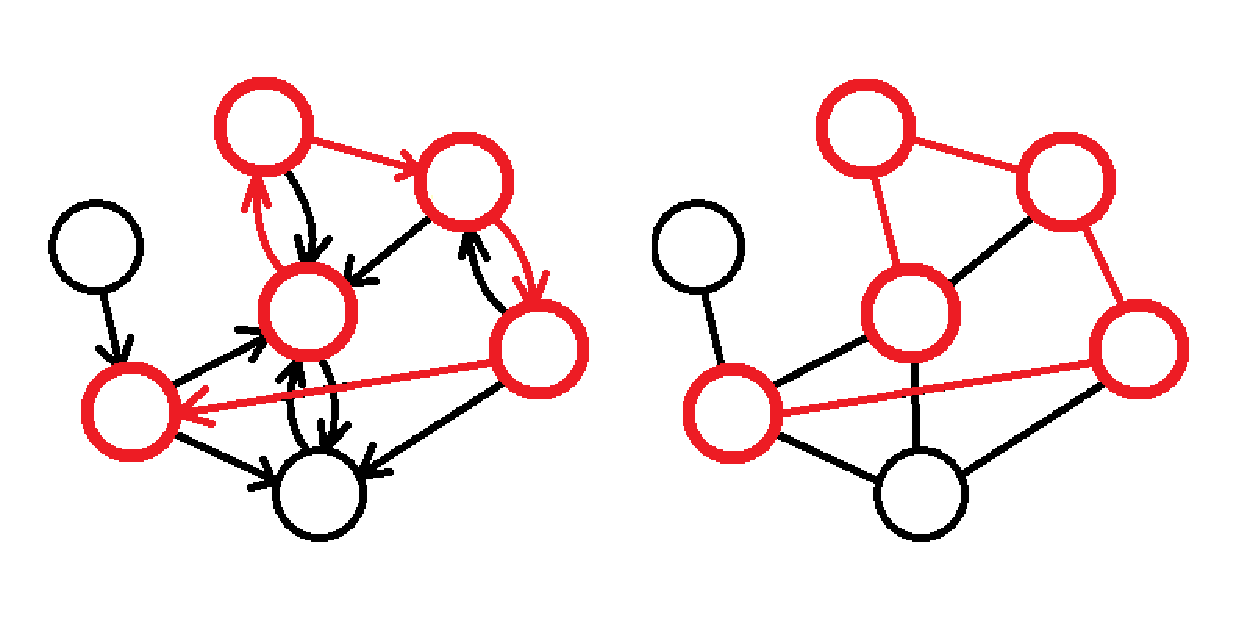
\includegraphics[width=8cm]{image/graph06.pdf}
    }
  \end{exampleblock}
}

\subsection{閉路}
\frame{
  \frametitle{閉路}
  \begin{block}{circuit}
    グラフ$G$の歩道$W = v_1, e_1, v_2, \cdots, v_k, e_k, v_{k+1}$が\\
    $v_1 = v_{k+1}$を満たすとき,$W$を$G$の閉路という.
  \end{block}
}

\subsection{連結}
\frame{
  \frametitle{連結}
  \begin{block}{connected}
    無向グラフ$G$の任意の頂点の組$v,w$について,\\
    $v$と$w$を結ぶ道が存在するとき,$G$は連結であるという.
  \end{block}
}

\frame{
  \begin{exampleblock}{連結グラフと非連結グラフ}
    左が連結グラフ,右が非連結グラフ
    \center{
      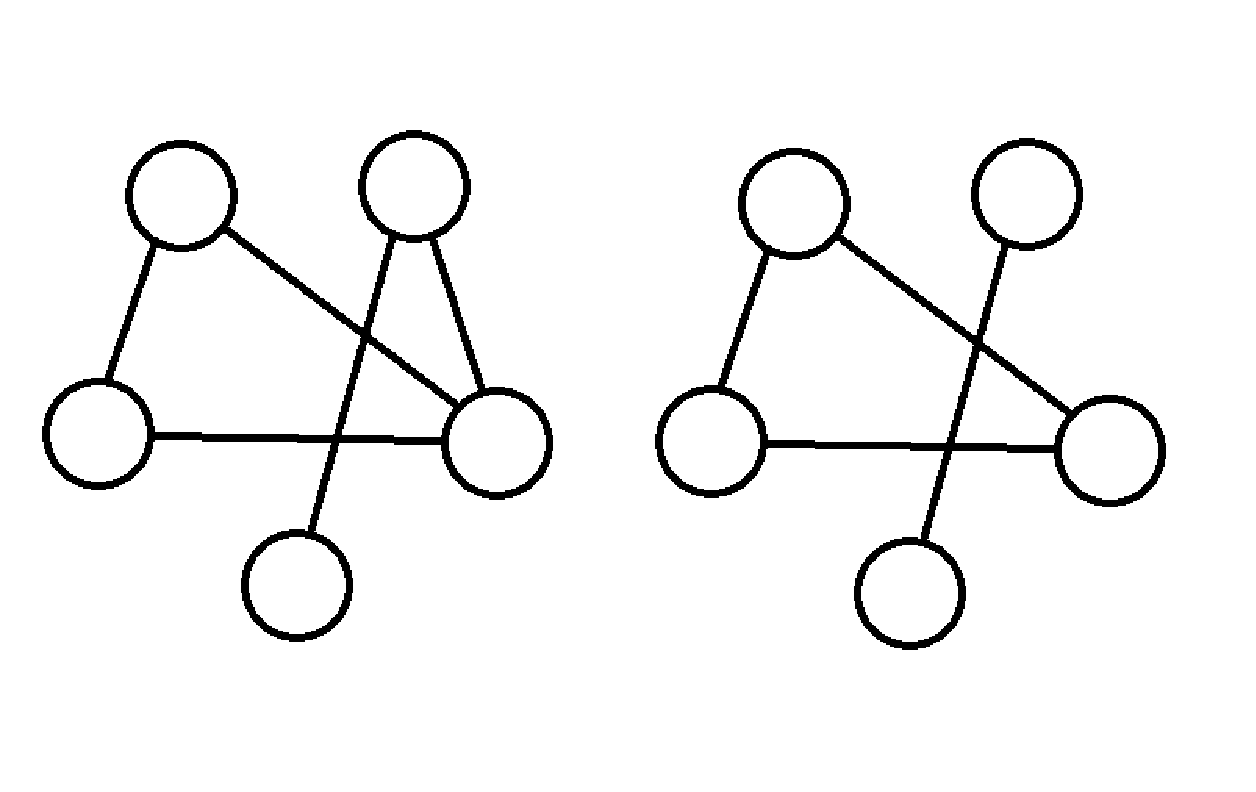
\includegraphics[width=8cm]{image/graph07.pdf}
    }
  \end{exampleblock}
}

\subsection{What's 木?}
\frame{
  \frametitle{木}
  \begin{block}{tree}
    無向グラフ$G$が連結であり閉路が存在しないとき,\\
    $G$を無向木という.
  \end{block}
  \begin{block}{arborescence}
    有向グラフ$G$に閉路が存在せず,1つの頂点を除いて\\
    他の全ての頂点の入次数が1のとき,$G$を無向木という.
  \end{block}
}

\frame{
  \begin{exampleblock}{木の例}
    左が無向木,右が有向木
    \center{
      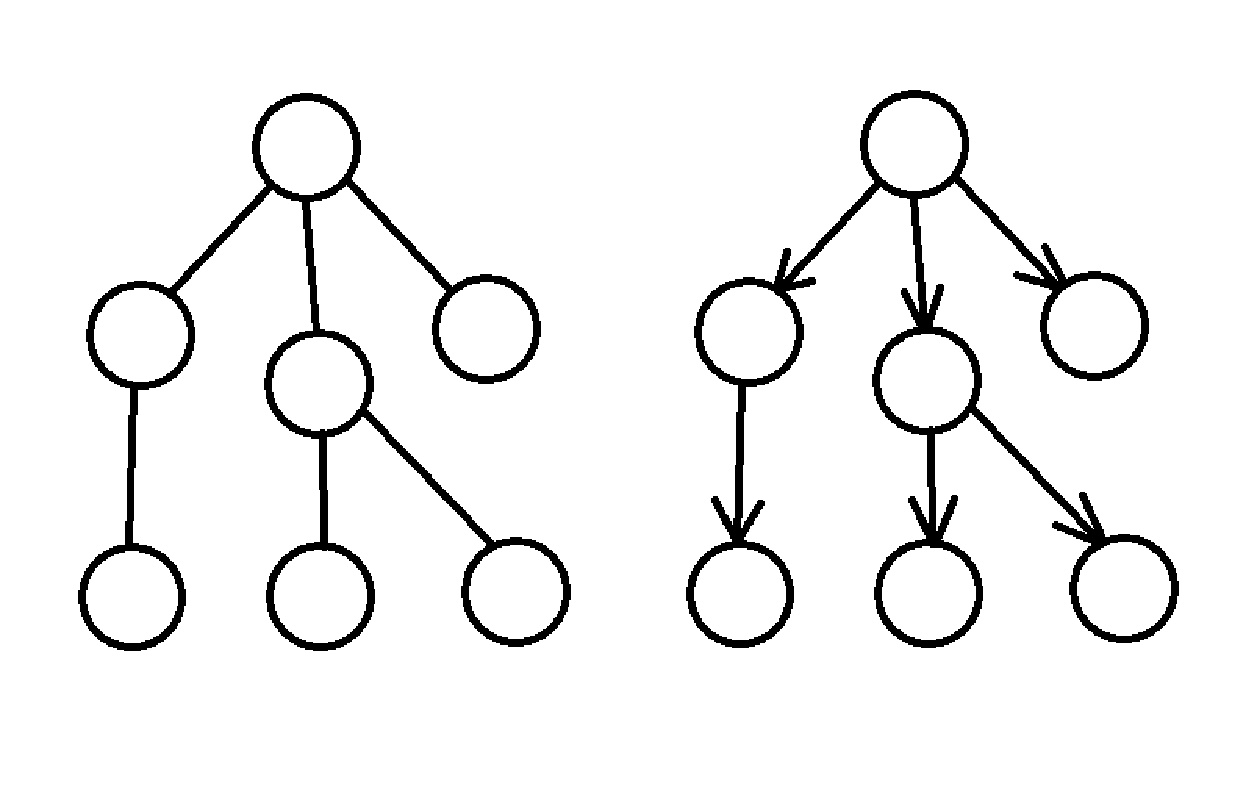
\includegraphics[width=8cm]{image/graph08.pdf}
    }
  \end{exampleblock}
}

\frame{
  という感じで厳密な定義を講義したかった\\ \\
  \pause
  しかし,講義時間は限られている (5時間よこせ
}

\frame{
  \frametitle{これが木だ!!!!11}
  \begin{exampleblock}{有向木}
    \center{
      図略
       \\
      根が1つだけ存在する.\\
      根以外の頂点は,親を1つだけ持つ.\\
      ループは存在しない\\
    }
  \end{exampleblock}
}
